%The RDF bipartite graph introduced in Section~\ref{sec:graph-rep-for-rdb}, Chapter~\ref{chap:representation}, can preserve the semantics of data and, unlike other alternative representations, induces no ambiguity.
The RDF bipartite graph is able to represent data and domain knowledge encoded in ontologies in the same way so that analysis approaches on the RDF bipartite graph can benefit from the combined source of information. In the last chapter, we describe in detail the mining method for cases where ontologies are not necessary to be included based on the coarsened RDF hypergraphs. In this chapter, we cover cases where ontologies are present and incorporated so that mining semantically associated itemsets can be more effective with the help of encoded domain knowledge.

This chapter makes the following main contributions:  First, we employ the RDF bipartite graph representation to capture both ontologies and data. We can weight each edge so that certain links (such as \emph{is\_a} or \emph{may\_treat} relationships) can carry appropriate strength.  Then, we implement highly efficient and scalable random walks with restart over the RDF bipartite graph to generate semantically associated itemsets. Finally, we evaluate the correctness of the results on well-known shopping cart datasets, and the scalability of the method on our large electronic healthcare dataset.
\section{Method}
%Mining Semantically Associated Itemsets with the Incorporation of Ontologies

To enable the incorporation of ontologies in mining semantically associated itemsets, we use the RDF bipartite representation described in Chapter~\ref{chap:representation}. We distinguish different semantic relationships in the RDF bipartite graph by assigning weights to those corresponding paths. The various semantic relationships include, for example,  class subsumption, part\_of, and other general or domain--specific properties.

Formally, the RDF bipartite graph as a combined representation for both data and ontologies is defined as $G=\langle V_v \cup V_s, E \rangle$, where $V_v$ denotes \emph{value nodes} corresponding to components of RDF statements (\ie, subject, predicate, or object), and $V_s$ denotes \emph{statement nodes} corresponding to RDF statements. More specifically, statement nodes can be further divided according to whether they are from data or ontology, \ie, $V_s=V_d \cup V_o$; Value nodes can be divided according to whether they represent rows (records) or columns (attributes) in data, \ie, $V_d=V_r \cup V_a$. The graph $G$ can be represented in a biadjacency matrix $\mathbf{M}$, where $\mathbf{M}(i,j)$ is non-zero if there is an edge between $\langle V_{v_i}, V_{s_j} \rangle$. For an unweighted graph, the value can be 0/1, and for a weighted graph, any non-negative value.

\begin{myexp}[\textbf{An example RDF bipartite graph and its biadjacency matrix}]
\label{ex:bi-adj}
In Figure~\ref{fig:biadjacency-matrices} we show an example of an RDF bipartite graph. This graph has been used in Chapter~\ref{chap:representation} to demonstrate how a data graph and an ontology graph can be combined into a single RDF bipartite graph. In this example, we describe its biadjacency matrix. The upper half of the bipartite graph in Figure~\ref{fig:biadjacency-matrices}(A) is constructed from information of a domain ontology, which is corresponding to RDF statements $s_1$--$s_4$ in Figure~\ref{fig:biadjacency-matrices}(B). The lower half of the bipartite graph is from a transaction table, which can be represented by statements $s_5$--$s_{12}$. Figure~\ref{fig:biadjacency-matrices}(C) shows the biadjacency matrices $\mathbf{M}_d$ and $\mathbf{M}_o$ for the data and ontology part of the RDF bipartite graph respectively. We can see that rows of $\mathbf{M}_d$ and $\mathbf{M}_o$ correspond to \emph{value nodes}, ($V_v$), which can be further divided into row nodes $V_r$ and attribute nodes $V_a$. On the other hand, columns of $\mathbf{M}_d$ are nodes that correspond to RDF statements about data ($V_d$), and columns of $\mathbf{M}_o$ correspond to the ontology ($V_o$). The union of $V_d$ and $V_o$ constitutes the whole set of statement nodes $V_s$ (circle nodes in Figure~\ref{fig:biadjacency-matrices}(A).
\end{myexp}


\begin{figure}[h!t]
\begin{center}
\begin{tabular}{c  c}
\multirow{12}{*}{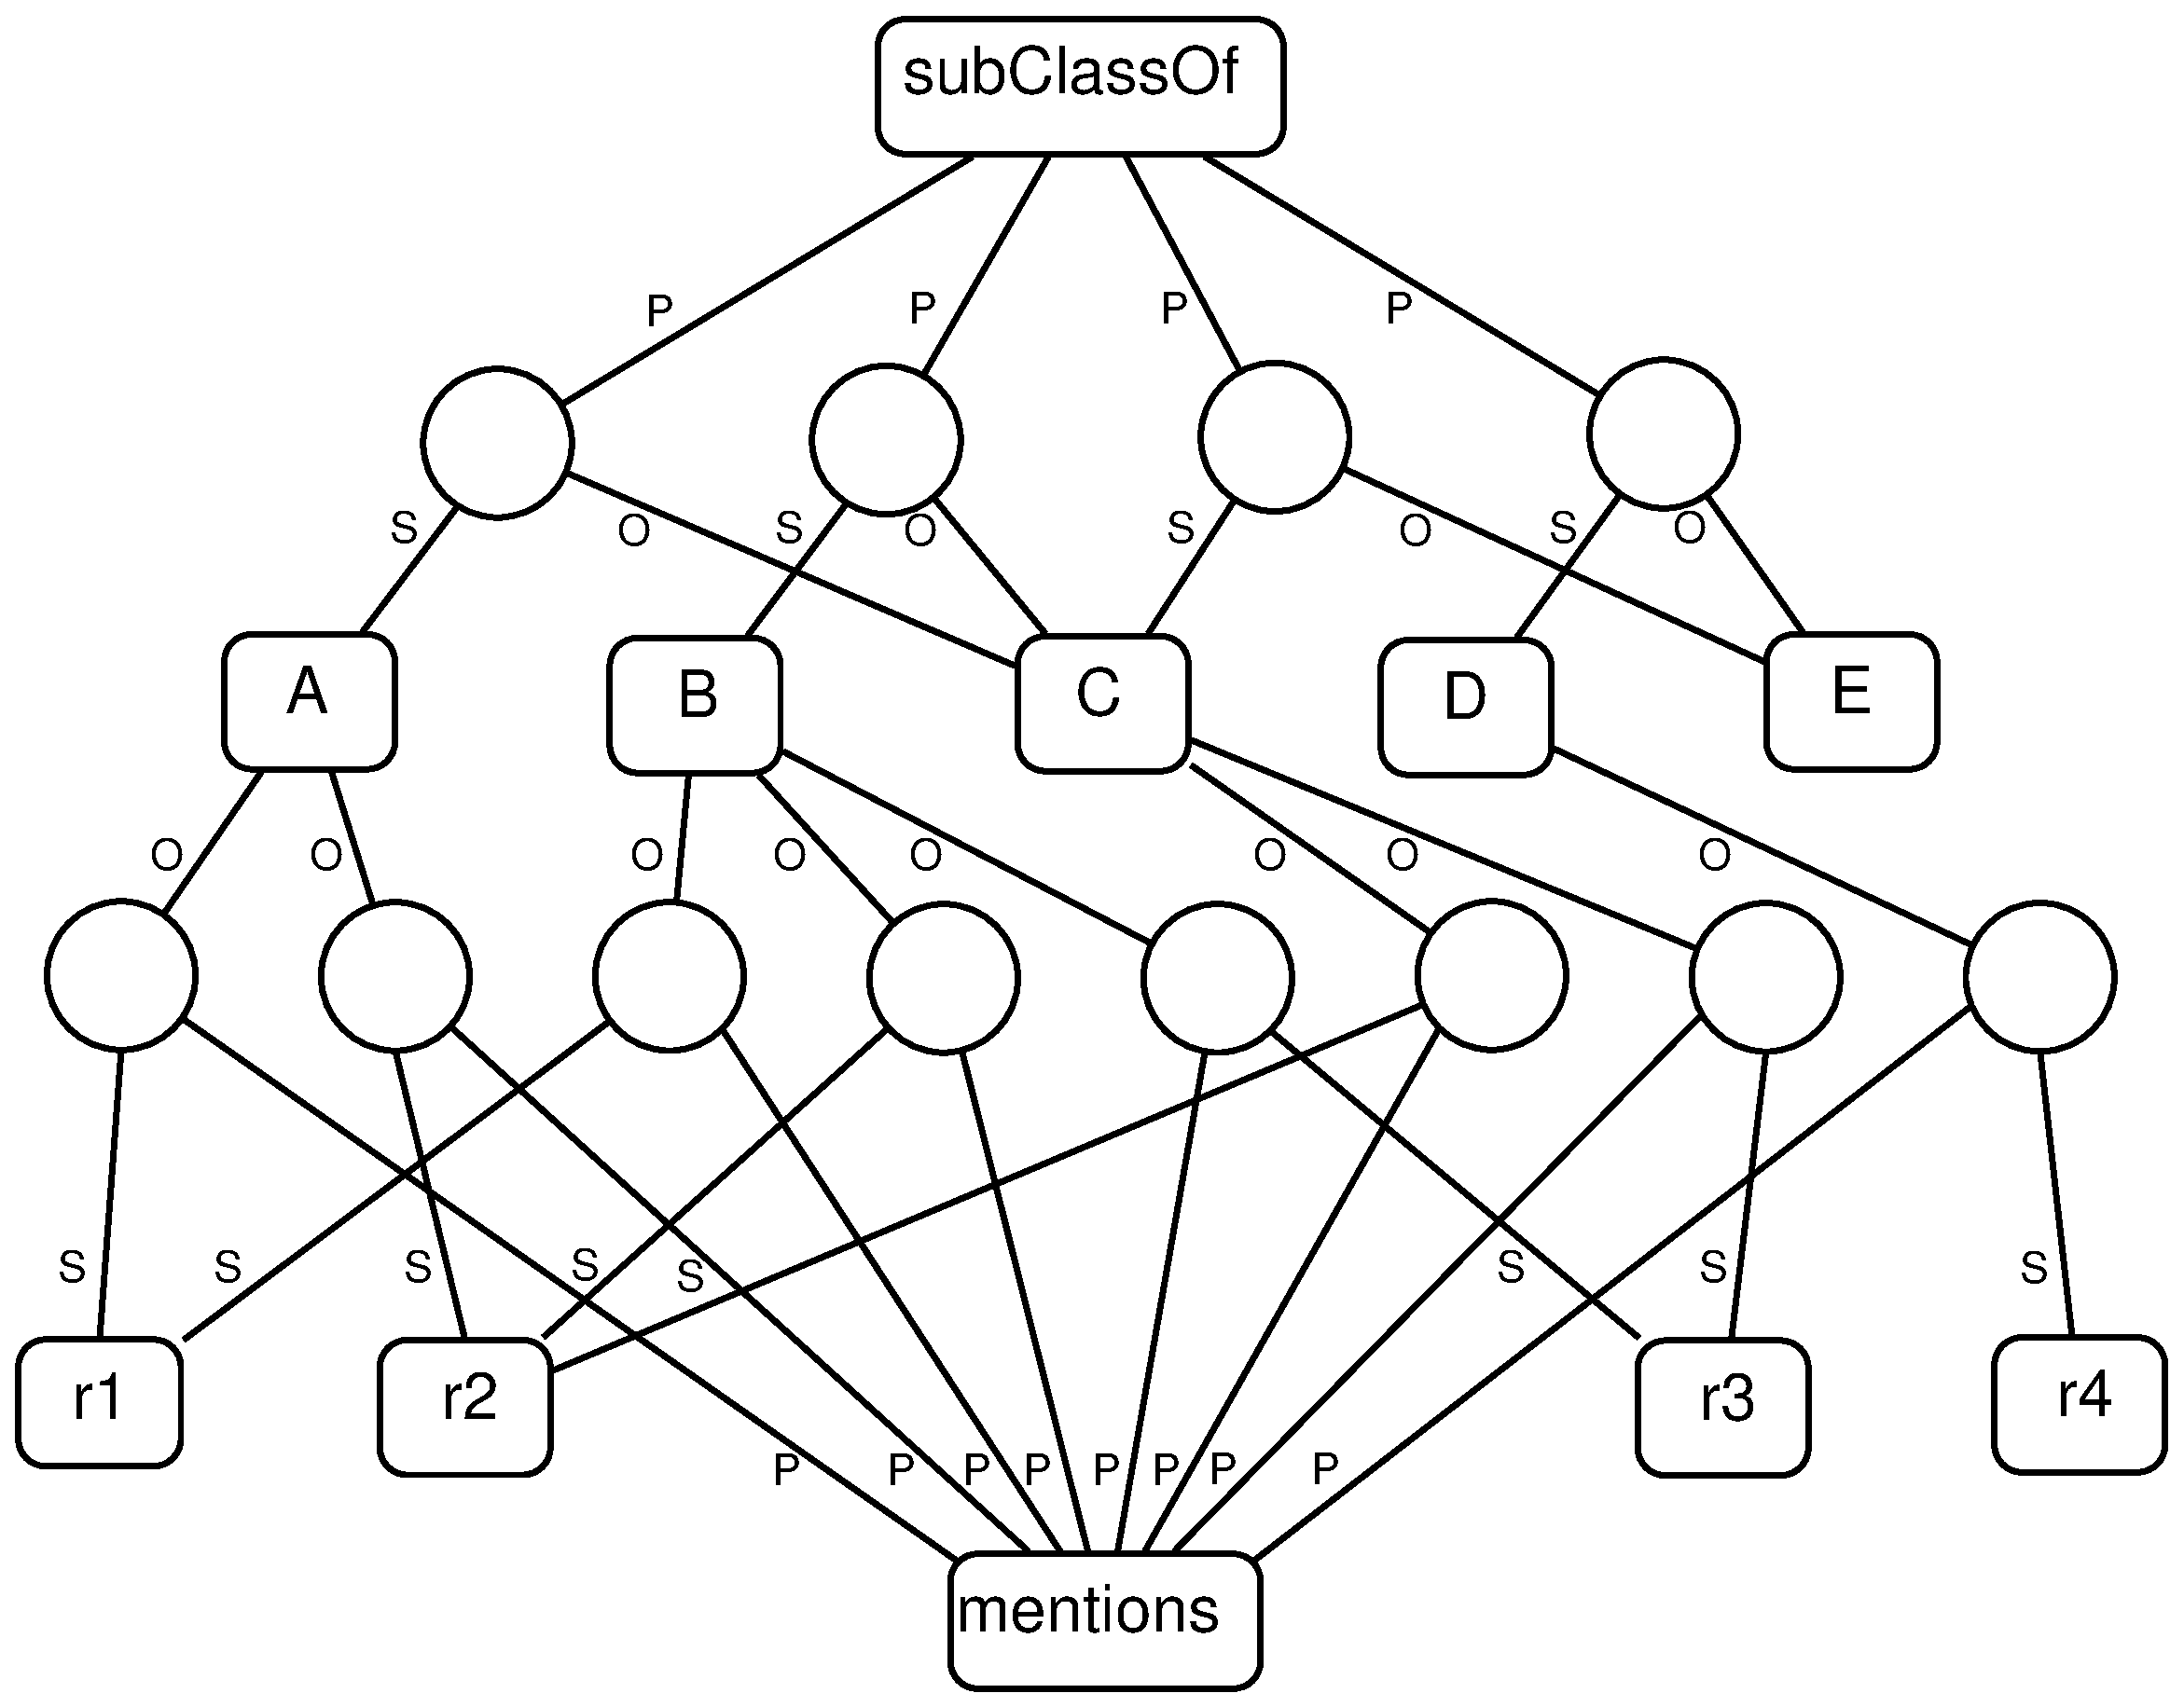
\includegraphics[width=.55\textwidth]{fig/hypergraph_mining.eps}} & {~~~~~~~~~~~~S \hfill P\hfill O~~~~~~~~}\\
& $s_1$:~~~\texttt{<A>~~<subClassOf>~~<C>}\\
& $s_2$:~~~\texttt{<B>~~<subClassOf>~~<C>}\\
& $s_3$:~~~\texttt{<C>~~<subClassOf>~~<E>}\\
& $s_4$:~~~\texttt{<D>~~<subClassOf>~~<E>}\\
& \\
& $s_5$:~~~\texttt{<r1>\;~~<mentions>\;~~<A>}\\
& $s_6$:~~~\texttt{<r1>\;~~<mentions>\;~~<B>}\\
& $s_7$:~~~\texttt{<r2>\;~~<mentions>\;~~<A>}\\
& $s_8$:~~~\texttt{<r2>\;~~<mentions>\;~~<B>}\\
& $s_9$:~~~\texttt{<r2>\;~~<mentions>\;~~<C>}\\
& $s_{10}$:~~\texttt{<r3>\;~~<mentions>\;~~<B>}\\
& $s_{11}$:~~\texttt{<r3>\;~~<mentions>\;~~<C>}\\
& $s_{12}$:~~\texttt{<r4>\;~~<mentions>\;~~<D>}\\
& \\
& \\
(A) & (B)\\
\multicolumn{2}{c}{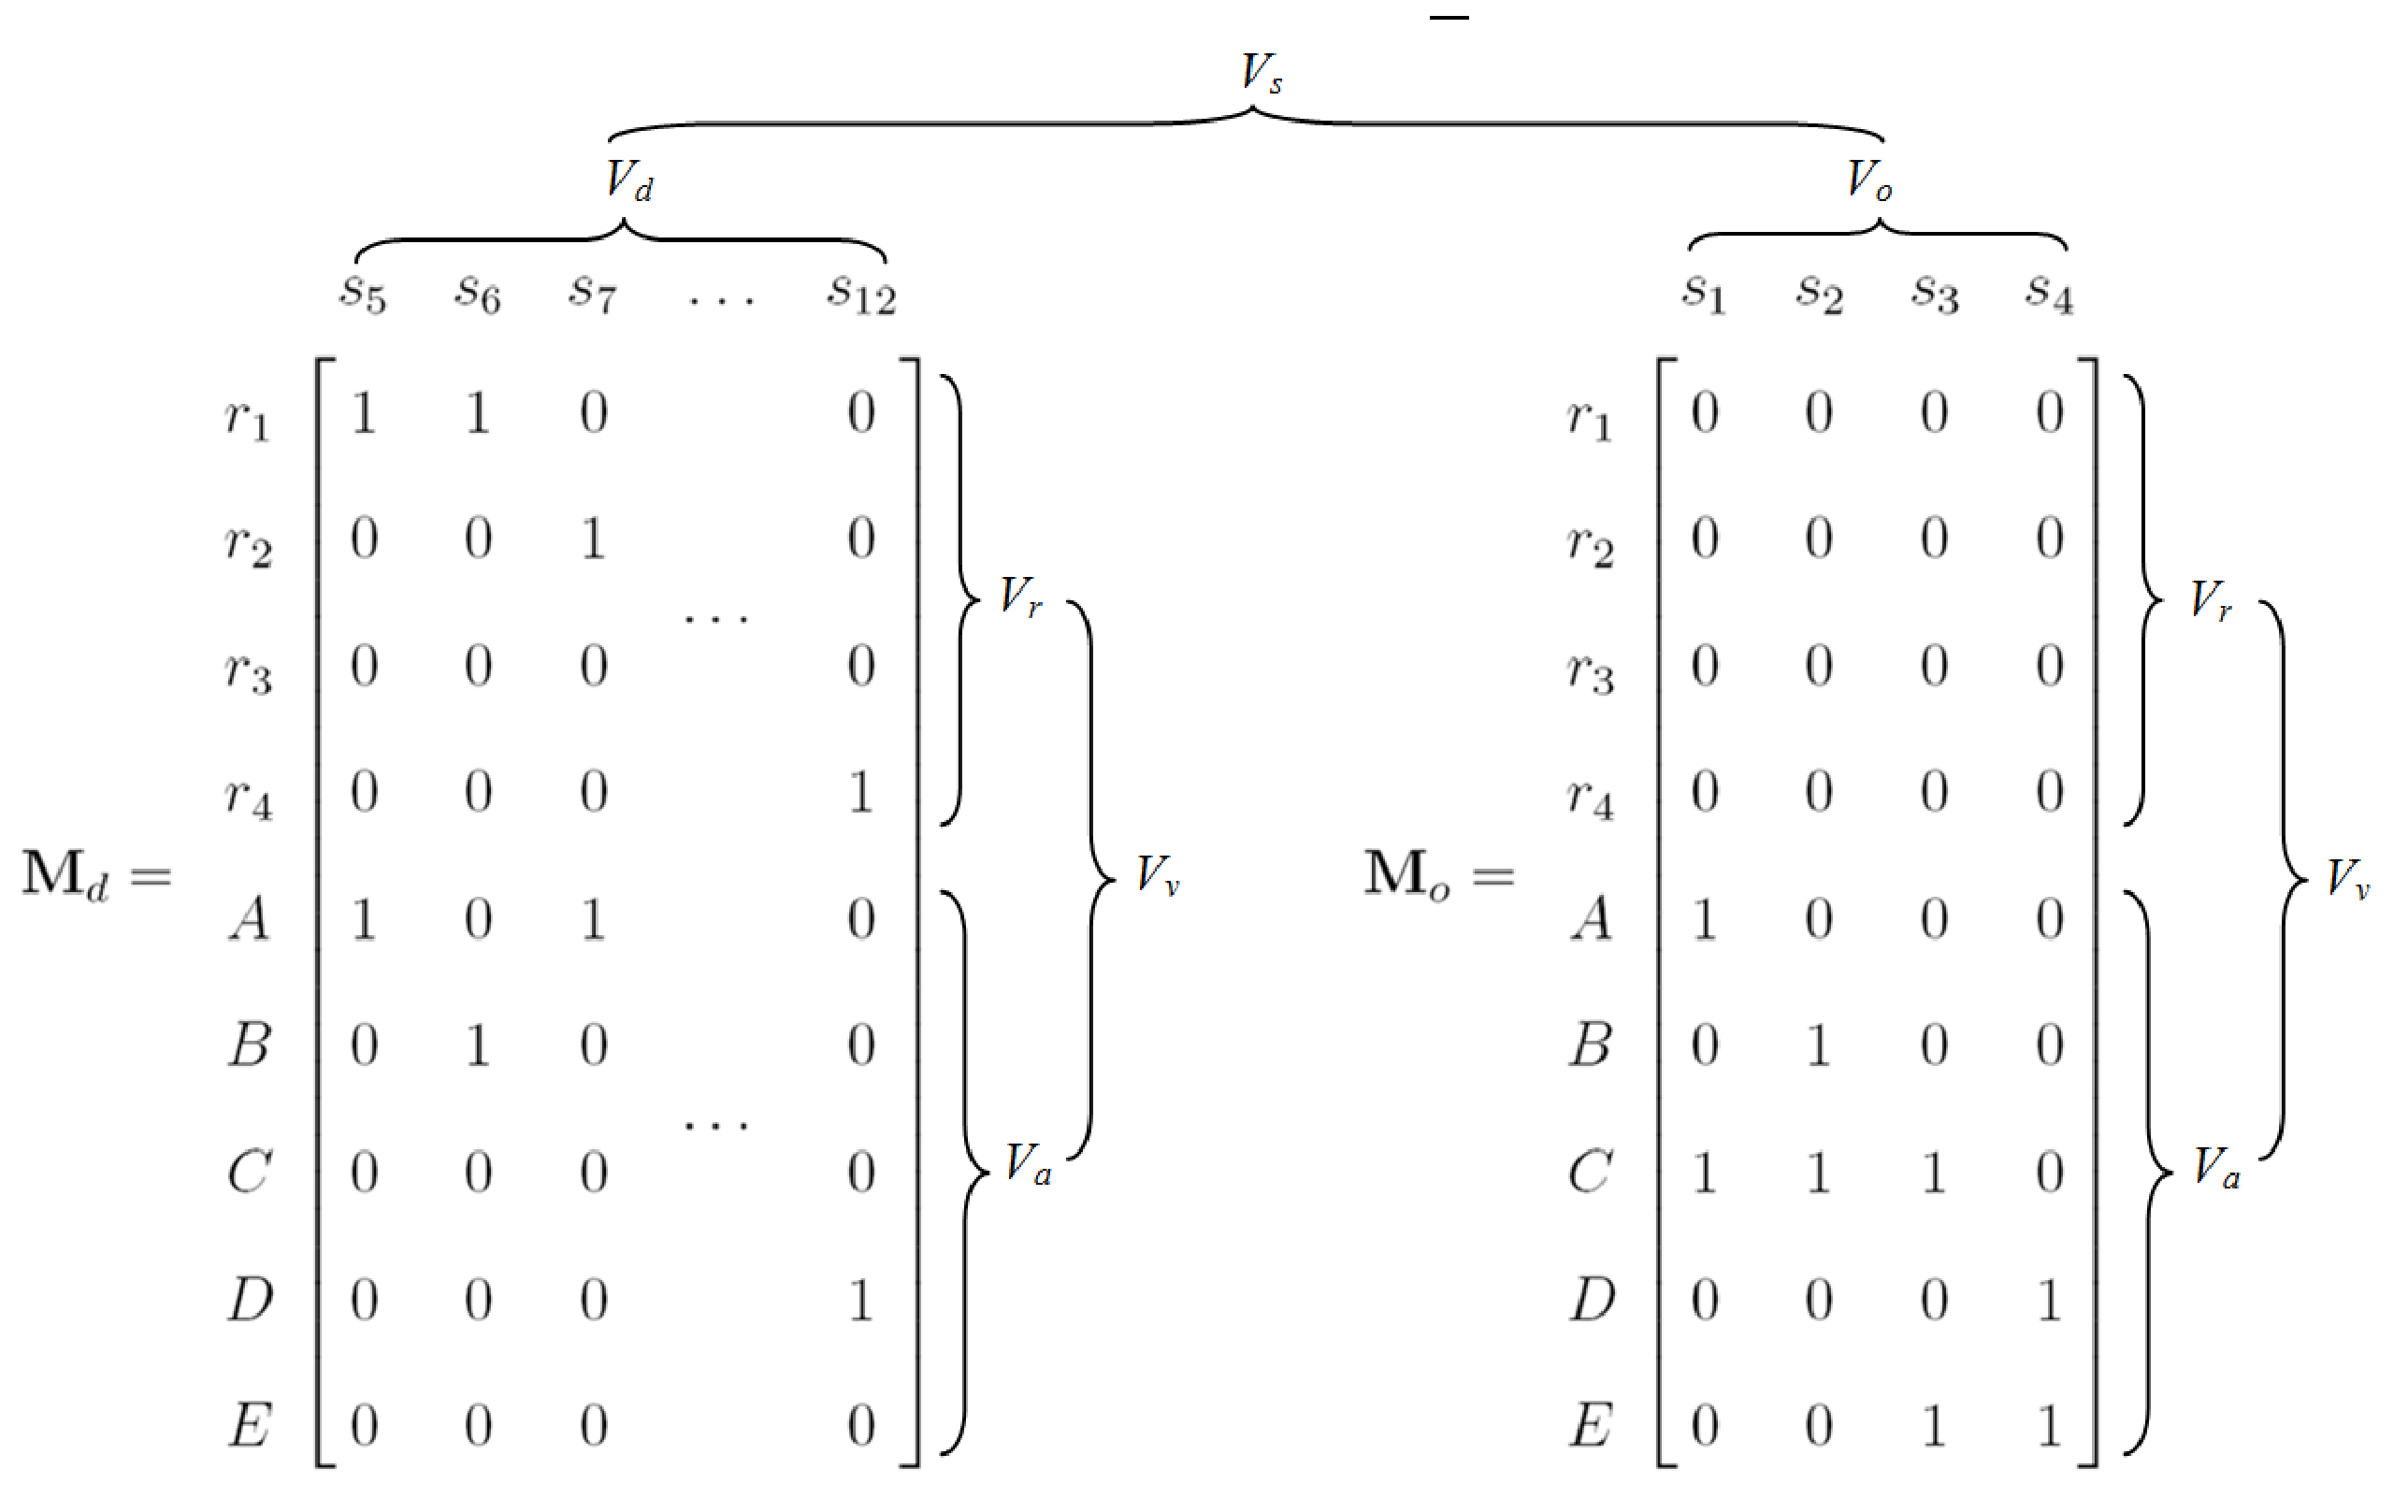
\includegraphics[width=\textwidth]{fig/biadjacency-matrices.eps}}\\
\multicolumn{2}{c}{(C)}
\end{tabular}
\end{center}
\caption[An example RDF bipartite graph and its biadjacency matrix]{\label{fig:biadjacency-matrices} An example RDF bipartite graph and a detailed anatomy of its biadjacency matrix.}
\end{figure}
\clearpage

From this example we notice that the biadjacency matrix $\mathbf{M}$ can be split into vertical stripes by statement nodes $V_s$. To obtain the biadjacency matrix $\mathbf{M}$ of the combined RDF bipartite graph in Figure~\ref{fig:biadjacency-matrices}(A), we can simply concatenate $\mathbf{M}_d$ and $\mathbf{M}_o$ horizontally: $\mathbf{M}=\left[\mathbf{M}_d~\mathbf{M}_o\right]$. This gives us a way to construct the matrix modularly from its independent components. In general, if there are $k$ different semantic relationships in ontologies, $\mathbf{M}_o$ can be divided into more vertical stripes $\{\mathbf{M}_{o_i}, i=1\dots k\}$, where $\mathbf{M}_{o_i}$ may represent, for example, the ``part\_of" lattice. Each $\mathbf{M}_{o_i}$ can be distinguished from others by different weights assigned to it. In short, $\mathbf{M}$ is the horizontal concatenation of all weighted vertical stripes as shown in~\ref{eq:horzcat}. The internal block structure of the concatenated biadjacency matrix $\mathbf{M}$ is shown in~\ref{striped_M}.

%horizontal concatenation
\begin{equation}\label{eq:horzcat}
\mathbf{M} = \bigg[w_d\mathbf{M}_d ~~ w_{o_1}\mathbf{M}_{o_1} ~~ w_{o_2}\mathbf{M}_{o_2} ~~ \dots\bigg]
\end{equation}

\begin{equation}
\label{striped_M}
\mathbf{M}=\begin{blockarray}{ccccc}
                ~ & ds & os_1 & os_2 & \dots \\
            \begin{block}{c[c|c|c|c]}
                r   &   \mathbf{M}_{dr}  &   \mathbf{0}   &   \mathbf{0}   &   \dots \\
                \cline{2-5}
                a   &   \mathbf{M}_{da}  &   \mathbf{O}_1 &   \mathbf{O}_2 &   \dots \\
            \end{block}
        \end{blockarray}
\end{equation}

%By developing the unified representation for both data and domain knowledge, and utilizing ontology annotations (\eg,~\cite{LePendu2010}), we can produce a unified RDF bipartite graph, which serves as the basis for mining semantically associated itemsets. With additional information from domain knowledge encoded in ontologies, the unified RDF bipartite graph enables us to discover interesting indirect relationships between entities from data. Moreover, the same method also makes it possible to validate relationships between ontological concepts with the help of the present data graph. In the next section, we describe a similarity measure based on random walk with restart on the RDF bipartite graph to capture the semantic association.

With the RDF bipartite graph and the form of its biadjacency matrix defined, in the next section, we move on to describe a similarity measure based on random walk with restart over this graph to discover semantically associated itemsets.


\subsection{Similarity Ranking by Random Walk with Restart}

Similar to the relevance score~\cite{SunEtal05}, we believe that two items have a strong semantic association if they are related to many similar objects. We denote the similarity score between entities $e_1$ and $e_2$ by $s(e_1, e_2)$, where $s(e_1,e_2) \in [0, 1]$ and $s(e_1, e_2) = 1 \text{ if } e_1 = e_2$. Now the problem of ranking semantic associations in the unified graph can be described as follows.

Given an attribute node $a$ in the unified graph $G = G_d \cup G_o$ and $a \in G_d \cap G_o$ we want to compute a similarity score $s(a, b)$ for all nodes $b(\neq a) \in G_d \cap G_o$. The result is a one-column vector containing all similarity scores with respect to $a$~\cite{Chen_tuplerank:ranking}. We choose to apply random walks with restart (RWR) from the given node $a$, and use the steady-state probability of each other node at convergence as the similarity measure. In other words, the similarity score of node $b$ is defined as the probability of visiting $b$ via a random walk which starts from $a$ and goes back to $a$ with a probability $c$.

RWR is closely related to the two similarity measures, \ie, $s_{CT}$ and $s_{L+}$, that are presented in Chapter~\ref{chap:datamining} on RDF hypergraphs, since they are all derived from the random walk model. It is sometimes a desirable property of a similarity measure for many applications, if it is able to discount nodes with large degrees like the $s_{L+}$ measure. The adaptation of $s_{L+}$ to RDF bipartite graph is a topic worth exploring in future work. However, the scores of RWR on bipartite graphs are easier to compute, especially, when the number of nodes in the two sides is highly unbalanced. The RDF bipartite graph is unbalanced because there are generally many more statement nodes than value nodes on large graphs. Therefore we focus on studying RWR over the RDF bipartite graph in this chapter.

In more detail, RWR in a bipartite graph works as follows: assume we have a random walker that starts from node $a$. For each step, the walker chooses randomly among the available edges from the current node. After each iteration, with probability $c$, it resets its position back to node $a$. The final steady-state probability that the random walker reaches node $b$ is the similarity score of $b$ with respect to $a$. We choose the random walk approach to compute the relevance score because it gives node $b$ high ranking if $b$ and $a$ are connected by many nodes; this is due to the random walker having more paths to reach $b$ from $a$. The purpose of the periodic restart of the random walk is to raise the chance that close related nodes are visited more often than other nodes.

In the following, we describe how to calculate algorithmically the similarity ranking based on random walk with restart on the unified RDF bipartite graph. The algorithm can be used in situations where, for example, users are interested in knowing products that are usually bought together in the same transactions by different customers, or common side effects of the same drugs prescribed to different patients, etc.

Given a biadjacency matrix $\mathbf{M}$ in~\ref{eq:horzcat} for the combined RDF bipartite graph $G$, we can construct the adjacency matrix $\mathbf{A}$ of $G$ as following:
\[
\mathbf{A}=\left[
               \begin{array}{cc}
                 \mathbf{0}   & \mathbf{M} \\
                 \mathbf{M}^T & \mathbf{0} \\
               \end{array}
             \right].
\]
The probability of a random walker taking a particular edge $\langle a,b\rangle$ from a node $a$ while traversing the graph is proportional to the edge weight over the total weight of all outgoing edges from $a$, i.e., $\mathbf{P}(a,b)=\mathbf{A}(a,b)/\Sigma_{i=1}^{m+n}\mathbf{A}(a,i)$. Therefore, the Markov transition matrix $\mathbf{P}$ of $G$ is constructed as: $\mathbf{P}=normc(\mathbf{A})$, where $normc(\mathbf{A})$ normalizes $\mathbf{A}$ such that every column sum up to 1.

Given the transition matrix $\mathbf{P}$, we can calculate the similarity scores using the following steps. First, we transform the input attribute node $a$ into a $(k+n) \times 1$ query vector $\mathbf{q}_a$ with 1 in the $a$-th row and 0 otherwise. Second, we need to compute a $(k+n)\times 1$ steady-state probability vector $\mathbf{u}_a$ over all nodes in $G$. Last we extract only the steady-state probabilities of row nodes in $\mathbf{M}$ (corresponding to value nodes in the RDF bipartite graph) as the output similarity score vector. Notice that $\mathbf{u}_a$ can be computed by an iterated method from the following iterative equation.

Let $c$ be the probability of restarting random-walk from the node $a$. Then the steady-state probability vector $\mathbf{u}_a$ satisfies
\begin{equation}
\label{eq:steady-state}
\mathbf{u}_a=(1-c)\mathbf{P}_A\mathbf{u}_a+c\mathbf{q}_a~.
\end{equation}

\renewcommand{\algorithmicrequire}{\textbf{Input:}}
\renewcommand{\algorithmicensure}{\textbf{Output:}}
\begin{algorithm}
\caption{Calculate Semantic Association}
\label{alg1}
\begin{algorithmic}
\REQUIRE query attribute $a$, bipartite matrix $M$, restarting probability $c$, tolerant threshold $\epsilon$
\ENSURE similarity vector $\mathbf{u}_a(1:k)$
\STATE $\mathbf{q}_a \Leftarrow \mathbf{0}$
\STATE $\mathbf{q}_a(a)=1$ (set $a$-th element of $\mathbf{q}_a$ to 1)
\WHILE{$|\Delta\mathbf{u}_a| > \epsilon$}
\STATE \[
    \mathbf{u}_a = (1-c)  \left[ \begin{array}{c}
        normc(\mathbf{M})\mathbf{u}_a(k+1:k+n);\\
        normc(\mathbf{M}^T)\mathbf{u}_a(1:k)
    \end{array} \right] + c\mathbf{q}_a
\]
\ENDWHILE
\RETURN $\mathbf{u}_a(1:k)$
\end{algorithmic}
\end{algorithm}

The iterative update of $\mathbf{u}_a$ can be performed as shown in Algorithm~\ref{alg1}. The while loop is modified from~\ref{eq:steady-state} to avoid materializing $\mathbf{A}$ and $\mathbf{P}$ for scalability.


\section{Case Studies}
In this section, we evaluate the method of random walk with restart on the combined RDF bipartite graph for discovering semantic associations. We conducted a series of experiments to highlight the effect of the incorporating the ontologies in the mining task, and to explore the impact of different ratios of weights assigned to various kinds of relationships in the graph. First, to illustrate the power of combined RDF bipartite graph in finding semantic associations while taking into account seamlessly the ontological information, we evaluated our methods on a commonly used \emph{shopping cart} dataset together with a manually created ontology describing the subsumption hierarchy for grocery items.  Finally, we applied our method to actual \emph{electronic health records} to highlight its scalability and applicability to the medical domain.

Below we first summarize the sizes of the datasets used in our experiments in Table~\ref{tbl:exp_overview}.

\begin{table}[tbh]\scriptsize
\begin{center}
\begin{tabular}{c|c|c|c}
\hline
    & \# data stmts & \# isa stmts & \# other stmts$^\dag$ \\
    \hline
  Shopping cart     &  8,481       & 127       &    0\\
  Electronic health &  148,690,056  & 1,048,604 &    43780\\
  \hline
\end{tabular}
\end{center}
\caption[Overview of the test cases.]{\label{tbl:exp_overview} Dataset overview (``stmts" stands for RDF statements). $^\dag$ In the electronic healths test, we explore the ``may\_treat" relationship between drugs and diseases defined in the National Drug File.}
\end{table}


\subsection{Shopping Cart}
\subsubsection{Dataset}
The shopping cart dataset is the same as we used in the case study of Chapter~\ref{chap:datamining}. It contains purchase information on 100 grocery items (represented by boolean column headers) for 2,127 shopping orders (corresponding to tuples) from a Foodmart. We first construct an RDF bipartite graph from the dataset by transforming the table to 8481 RDF statements.

Besides, we manually create an ontology to organize the grocery items into a subsumption hierarchy. In this process, we introduce 28 parent nodes (the 100 grocery items appeared in the data are mostly at the leaf level) from which derive a total of 127 RDF statements. As the size of this dataset is fairly small, the calculation of similarity ranking for a given term is fast. In the following we highlight the effect of incorporation of ontology by comparing results obtained with and without ontologies.


\subsubsection{Results}
In Table~\ref{tbl:foodmart_comp}, results of items ranked by the strength of semantic association with regard to a query term ``Toothbrush" under various combinations of parameters are demonstrated side-by-side for comparison. We first show the result ranked by co-frequency in Table~\ref{tbl:foodmart_comp}(A) as a baseline. Then, we observe that without using ontology, performing random walk with restart on the data graph (Table~\ref{tbl:foodmart_comp}(A)) starting from ``toothbrush" yields similar results to the work reported in~\cite{LiuEtal11} based on random walk commute time similarity. Items ranked high in this setting where only the data graph is considered are typically either hub nodes (with many edges linking to other items) or co-frequent with the query item (many edges connecting them). Second, applying the same similarity ranking method solely on the ontology graph (Table~\ref{tbl:foodmart_comp}(C)) gives a list of association based on the graph-configuration of the ontological structure (in this case, the rdfs:subClassOf lattice). The items that are considered most similar to the query term ``Toothbrush" is its immediate parent class ``PersonalHygiene," followed by some most derived classes at the same level of ``PersonalHygiene" and then siblings of ``Toothbrush" itself. Next, Table~\ref{tbl:foodmart_comp}(D)--(F) demonstrate the results of mining on the combined graph with different ratios of weights assigned to ontology edges and data edges respectively. It is obvious that these results can be seen as a mix of the data-only and ontology-only results with various emphasis on the data or ontology. We can observe that when $w_o/w_d=20$ the ontology and data appear to have equal significance in determining the ranking ($w_o$ is the weight of ontology edges (\ie, rdfs:subClassOf) and $w_d$ is the weight of data edges). In a rough sense, it conforms to the ratio of the size of ontology graph and data graph as well (see Table~\ref{tbl:exp_overview}). In reality, the appropriate ratio for the edge weights is not only dependent on the size of graphs but also the specific configuration of the graph (depth, average degree, etc). Moreover, specifying the ratio of prior knowledge in ontologies and inductive evidences in data that one wants to employ for discovering new patterns is a highly empirical process. Multiple pilot trials may need to be carried out for the optimal ratio before it is applied to the real application.

\begin{table*}[tbh]\scriptsize
\begin{center}
\begin{tabular}{ c c || c c | c c }
\hline
\multicolumn{2}{c||}{ranked by co-frequency}&\multicolumn{2}{c|}{w/ data only}&\multicolumn{2}{c}{w/ ontology only}\\
\hline
item	&	freq	&	item	&	p(\%)	&	item	&	p(\%)	\\
\hline											
PaperWipes	&	8	&	Soup	&	0.42	&	PersonalHygiene	&	12.55	\\
Popcorn	&	7	&	Cookies	&	0.41	&	Snack	&	0.86	\\
Soup	&	6	&	NasalSprays	&	0.38	&	Health	&	0.64	\\
NasalSprays	&	6	&	Popcorn	&	0.32	&	Sponges	&	0.57	\\
Cookies	&	6	&	PaperWipes	&	0.29	&	Soap	&	0.57	\\
Spices	&	5	&	FrozenVegetables	&	0.29	&	Shampoo	&	0.57	\\
Soda	&	4	&	PersonalHygiene	&	0.26	&	NasalSprays	&	0.57	\\
Shrimp	&	4	&	DriedFruit	&	0.25	&	Mouthwash	&	0.57	\\
FlavoredDrinks	&	4	&	Milk	&	0.25	&	Conditioner	&	0.57	\\
Dips	&	4	&	Mouthwash	&	0.24	&	MealCourse	&	0.54	\\
\hline
\multicolumn{6}{c}{~}\\
\multicolumn{2}{c}{(A)}  &   \multicolumn{2}{c}{(B)}  &   \multicolumn{2}{c}{(C)}  \\
\multicolumn{6}{c}{~}\\
\end{tabular}

\begin{tabular}{ c c | c c | c c }
\hline
\multicolumn{2}{c|}{$w_o=1$, $w_d=1$}&\multicolumn{2}{c|}{$w_o=10$, $w_d=1$}&\multicolumn{2}{c}{$o_w=20$, $o_d=1$}\\
\hline
item	&	p(\%)	&	item	&	p(\%)	&	item	&	p(\%)	\\
				\hline							
PersonalHygiene	&	0.74	&	PersonalHygiene	&	3.97	&	PersonalHygiene	&	6.27	\\
Soup	&	0.41	&	NasalSprays	&	0.41	&	NasalSprays	&	0.5	\\
Cookies	&	0.4	&	Soup	&	0.34	&	Mouthwash	&	0.41	\\
NasalSprays	&	0.37	&	Cookies	&	0.34	&	Shampoo	&	0.31	\\
Popcorn	&	0.31	&	Mouthwash	&	0.3	&	Soup	&	0.29	\\
FrozenVegetables	&	0.29	&	Popcorn	&	0.25	&	Cookies	&	0.29	\\
PaperWipes	&	0.28	&	FrozenVegetables	&	0.24	&	Sponges	&	0.28	\\
DriedFruit	&	0.25	&	PaperWipes	&	0.23	&	Health	&	0.27	\\
Milk	&	0.25	&	DriedFruit	&	0.22	&	Conditioner	&	0.27	\\
Mouthwash	&	0.23	&	Milk	&	0.21	&	Soap	&	0.25	\\
\hline
\multicolumn{4}{c}{~}\\
\multicolumn{2}{c}{(D)}  &  \multicolumn{2}{c}{(E)}  & \multicolumn{2}{c}{(F)}\\
\end{tabular}
\end{center}
\caption[Top results on the Foodmart dataset.]{\label{tbl:foodmart_comp} Foodmart items ranked by the strength of semantic association  (i.e., $p(\%)$, the steady-state probability), given the query term ``Tooth Brush."}
\end{table*}

We notice that without any filtering on the ranked semantic associations from the combined graph, the list includes items that never appear in the transactional data. This is because typically the semantic annotation process links table attributes to their most specific matching concept in the ontology which are close to the leaf level. The incorporation of ontology is to aid the mining process, therefore including in the result those parent nodes (\eg, ``PersonalHygiene") that never appear in the data is counterintuitive. To overcome this, we can simply filter out those items exclusive to the ontology. Table~\ref{tbl:foodmart_comp2} shows an example of filtered result given a query term ``soup." The co-frequency of items are also listed for comparison.

%Finally we tested our methods on the dataset of electronic health records of real patients. This dataset is different from the above two datasets not only in scale but also in practical importance as described in the following.
% state in very clear sentence what the conclusion is, what is the take-home message you want them to see? xxx

% why is this interesting? what should we have learned? xxx

%finally, lead-in to final experiment... we finally did this last experiment because:  1) its huge, 2) its important to people to solve xxx

\begin{table*}[tbh]\scriptsize
\begin{center}
\begin{tabular}{ c c c | c c c || c c c | c c c }
\hline
\multicolumn{6}{c||}{w/ data only}  &   \multicolumn{6}{c}{w/ onto only}\\
\hline
item	&	p(\%)	&	freq	&	item	&	p(\%)	&	freq	&	item	&	p(\%)	&	freq	&	item	&	freq	&	 p(\%)	 \\
\hline																							
Cheese	&	0.38	&	98	&	Preserves	&	0.19	&	65	&	TVDinner	&	0.46	&	40	&	Sponges	&	21	&	0.06	 \\
Cookies	&	0.32	&	96	&	Juice	&	0.17	&	47	&	Pizza	&	0.46	&	46	&	Soap	&	0	&	0.06	\\
DriedFruit	&	0.32	&	87	&	Lightbulbs	&	0.17	&	47	&	Pasta	&	0.46	&	29	&	Shampoo	&	34	&	0.06	 \\
Wine	&	0.24	&	63	&	PaperWipes	&	0.16	&	55	&	HotDogs	&	0.46	&	30	&	NasalSprays	&	21	&	0.06	 \\
CannedVegetables	&	0.23	&	67	&	Pizza	&	0.16	&	46	&	Hamburger	&	0.46	&	19	&	Mouthwash	&	28	 &	 0.06	 \\
FrozenVegetables	&	0.23	&	79	&	Nuts	&	0.16	&	60	&	FrenchFries	&	0.46	&	37	&	Conditioner	&	12	 &	 0.06	 \\
Cereal	&	0.22	&	56	&	Popcorn	&	0.16	&	39	&	DeliSalads	&	0.46	&	31	&	Ibuprofen	&	18	&	0.06	 \\
Milk	&	0.22	&	53	&	Chips	&	0.16	&	46	&	DeliMeats	&	0.46	&	37	&	ColdRemedies	&	33	&	 0.06	 \\
ChocolateCandy	&	0.19	&	16	&	Eggs	&	0.16	&	51	&	Sunglasses	&	0.07	&	12	&	Aspirin	&	22	&	 0.06	 \\
Waffles	&	0.19	&	51	&	TVDinner	&	0.15	&	40	&	Toothbrushes	&	0.06	&	13	&	Acetominifen	&	12	 &	 0.06	 \\
\hline
\end{tabular}
\end{center}
\caption[Top results on the Foodmart dataset excluding concepts only in the ontology.]{\label{tbl:foodmart_comp2} Semantically associated items  for the query term ``Soup," by filtering out those items exclusive to the Foodmart ontology.}
\end{table*}


\subsection{Electronic Health Records}
\subsubsection{Dataset}
In our second evaluation, we analyzed the electronic health records of real patients. The patient clinical note data are from Stanford Hospital's Clinical Data Warehouse (STRIDE). These records archive over 17-years worth of patient data comprising of 1.6 million patients, 15 million encounters, 25 million coded ICD9 diagnoses, and a combination of pathology, radiology, and transcription reports totaling over 9 million clinical notes (i.e., unstructured text).
We obtained the set of drugs and diseases for each patient's clinical note by using a new tool, the \emph{Annotator Workflow}, developed at the National Center for Biomedical Ontology (NCBO), which annotates clinical text from electronic health record systems and extracts disease and drug mentions from the electronic health records.

%In addition to having obvious data-mining applications, the workflow has been used by biomedical researchers to build semantic-search applications, such as the NCBO Resource Index~\cite{jonquet11}, which won the Semantic Web Challenge\footnote{\url{http://challenge.semanticweb.org/}} in 2010. The annotation process utilizes the vast NCBO BioPortal ontology library~\cite{bioportal} to extract information by using a lexicon of over one million terms generated from the relevant ontologies, such as SNOMED-CT, RxNORM, and MedDRA. Furthermore, it also incorporates negation detection --- the ability to discern whether a term is negated with the context of the narrative (e.g., lack of valvular dysfunction). Finally, it uses mappings between terms across ontologies~\cite{ghazvinian09}, which forms a rich knowledge graph %(Figure~\ref{fig:collapse})
%or mega-thesaurus, to normalize the lexicon by reducing the feature set from over one million to merely 11,107 unique drugs and 3,594 unique diseases.

From this set of 1.6 million patients with annotated records, we vectorize texts and turned them into a huge bag-of-word representation, from which an RDF bipartite graph is constructed (including 148 million RDF statements, see Table~\ref{tbl:exp_overview}). we applied our algorithms to all previous records in the patient's timeline, looking at just the set of drugs and their semantically related diseases.  Therefore, at a very simplistic level, the experiment result shows that strong semantically associated items in this context could possibly represent sets of drugs that could lead toward certain diseases.

One strength of the Annotator is the highly comprehensive and interlinked lexicon that it uses. It can incorporate the entire NCBO BioPortal ontology library of over 250 ontologies to identify biomedical concepts from text using a dictionary of terms generated from those ontologies. Terms from these ontologies are linked together via mappings. For this study, we specifically configured the workflow to use a subset of those ontologies that are most relevant to clinical domains, including Unified Medical Language System (UMLS) terminologies such as SNOMED-CT, the National Drug File (NDFRT) and RxNORM, as well as ontologies like the Human Disease Ontology. The resulting set of ontologies contains 1 million subsumption statements.

To highlight the capability of our method for incorporating multiple types of relationships, we also explore the ``may\_treat" relationship between drugs and diseases defined in NDFRT, for example, Thiabendazole may\_treat Larva Migrans. Since we are interested in learning the interaction between drugs and diseases, may\_treat is naturally a better indicator relationship to include while mining semantic associations than the subsumption relationship. Our results below illustrate this point.


\subsubsection{Results}
Before studying the drug-disease association, we carried out a similar test to that on the shopping cart dataset, in which we focus on studying the drug-drug and disease-disease association. To this purpose, we combine the subsumption hierarchy in the ontology graph with the data graph. Table~\ref{tbl:health_comp} shows the ranked semantic association for the query term ``Rofecoxib" (an active ingredient of some anti-inflammatory drugs) given different weight configuration to combine graphs. Without any preprocessing and prior knowledge about how the clinical notes are prescribed, the incorporation of subsumption relationship can be seen as a mean for denoising and enhancement of the data. Given the ratio of the size of the ontology to the size of data, the data graph in this test is more dominant in determining the ranking than in the shopping cart experiment. One can gradually change the ratio of $w_o$ to $w_d$ to strike a balance and achieve the optimal result.
\begin{table*}[tbh]\scriptsize
\begin{center}
\begin{tabular}{ c | c | c | c  }
\hline
rank    &   w/ data only	&	w/ onto only		&$w_o=10000, w_d=1$	 \\
\hline
1	&		reflux	&	valdecoxib	&		reflux	\\
2	&		medical history	&	meloxicam	&		obstruction	\\
3	&		history of previous events	&	celecoxib	&		injury	\\
4	&		diagnosis	&	parecoxib	&		valdecoxib	\\
5	&		pharmaceutical preparations	&	etoricoxib	&		medical history	\\
6	&		blood and lymphatic system disorders	&	deracoxib	&		foreign body sensation	\\
7	&		disease	&	lumiracoxib	&		history of previous events	\\
8	&		infantile neuroaxonal dystrophy	&	firocoxib	&		adverse effects	\\
9	&		today	&	nabumetone	&		celecoxib	\\
10	&		hypersensitivity	&	macrolides	&		actual hypothermia	\\
\hline
\end{tabular}
\end{center}
\caption[Top results on the electronic health dataset.]{\label{tbl:health_comp}Results of Health items ranked by the strength of semantic association, given the query term ``Rofecoxib."}
\end{table*}

To verify the drug--disease association and study the impact of different semantic relationships on finding such association, we carry out the following experiment. Table~\ref{tbl:health_exp} illustrates the rankings of three associations (one per row) under different settings. The first element in the pair is the query item, which are all active ingredients of some prescription drugs, and the ranking shown in the table is for the second item, which are diseases. For example, arthritis is ranked as the 527th semantically associated item to Rofecoxib according to similarity ranking based only on data graph. All these item pairs are actually gold standard associations backed by known drug--disease relationships, we know the strength of semantic associations between them should be strong.

We observe that the ranking based on data graph alone is fairly high already, consider there are approximately 1 million concepts of interest. However, the results based on the combination of data and subsumption (``isa") graph are worse. It is because the subsumption hierarchies for drugs and diseases are largely separate structures. Therefore the subsumption relationships can only boost the association within the drug and disease hierarchies respectively, but obfuscate the cross-hierarchy associations that we aim to find between drugs and diseases. On the other hand, however, the association between these pairs can be exactly captured by the NDFRT ``may\_treat" relationship (\eg, NDFRT explicitly defines that Rofecoxib may\_treat arthritis). When the ``may\_treat" graph is incorporated into the mining process, the ranking for the association is greatly boosted.

\begin{table*}[tbh]\scriptsize
\begin{center}
\begin{tabular}{ c || c  c || c  c || c  c }
\hline
        &   \multicolumn{2}{c||}{w/ data only}  &   \multicolumn{2}{c||}{w/ data and ``isa"} & \multicolumn{2}{c}{w/ data and ``may\_treat"}\\
\hline
\hline
                        	&   p(\%)   &   rank    &   p(\%)    &   rank    &   p(\%)    &    rank    \\
\hline
$\langle Rofecoxib, degenerative~polyarthritis\rangle$  &   0.006   &   527     &   0.004    &   632     &   0.51     &     13     \\
$\langle valdecoxib, degenerative~polyarthritis\rangle$  &   0.007   &   613     &   0.005    &   695     &   0.63     &     17     \\
$\langle troglitazone, diabetes\rangle$  &   0.006   &   478     &   0.005    &   514     &   0.44     &     11     \\
\hline
\end{tabular}
\end{center}
\caption{\label{tbl:health_exp}Rankings of three semantic associations in health data under different settings.}
\end{table*}





\begin{figure}[tbh]
\begin{minipage}[c]{0.49\textwidth}\centering
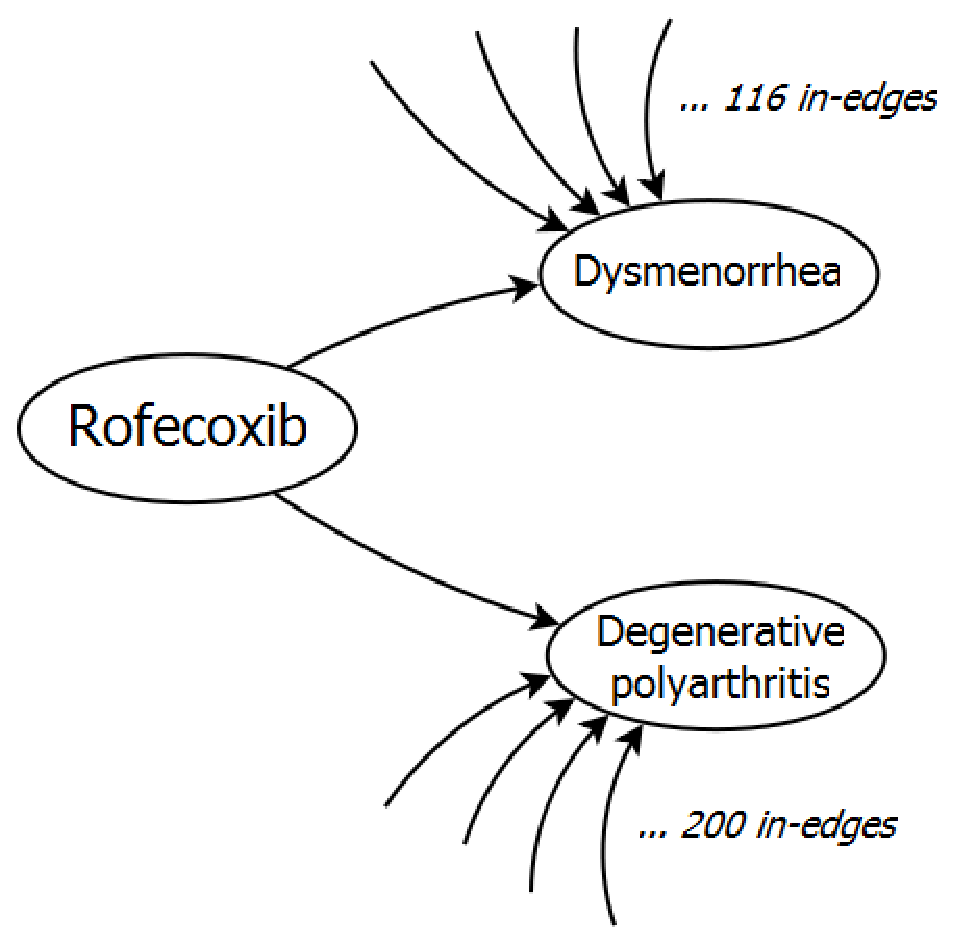
\includegraphics[width=.7\textwidth]{fig/may_treat.eps}
\end{minipage}
\begin{minipage}[c]{0.49\textwidth}\centering
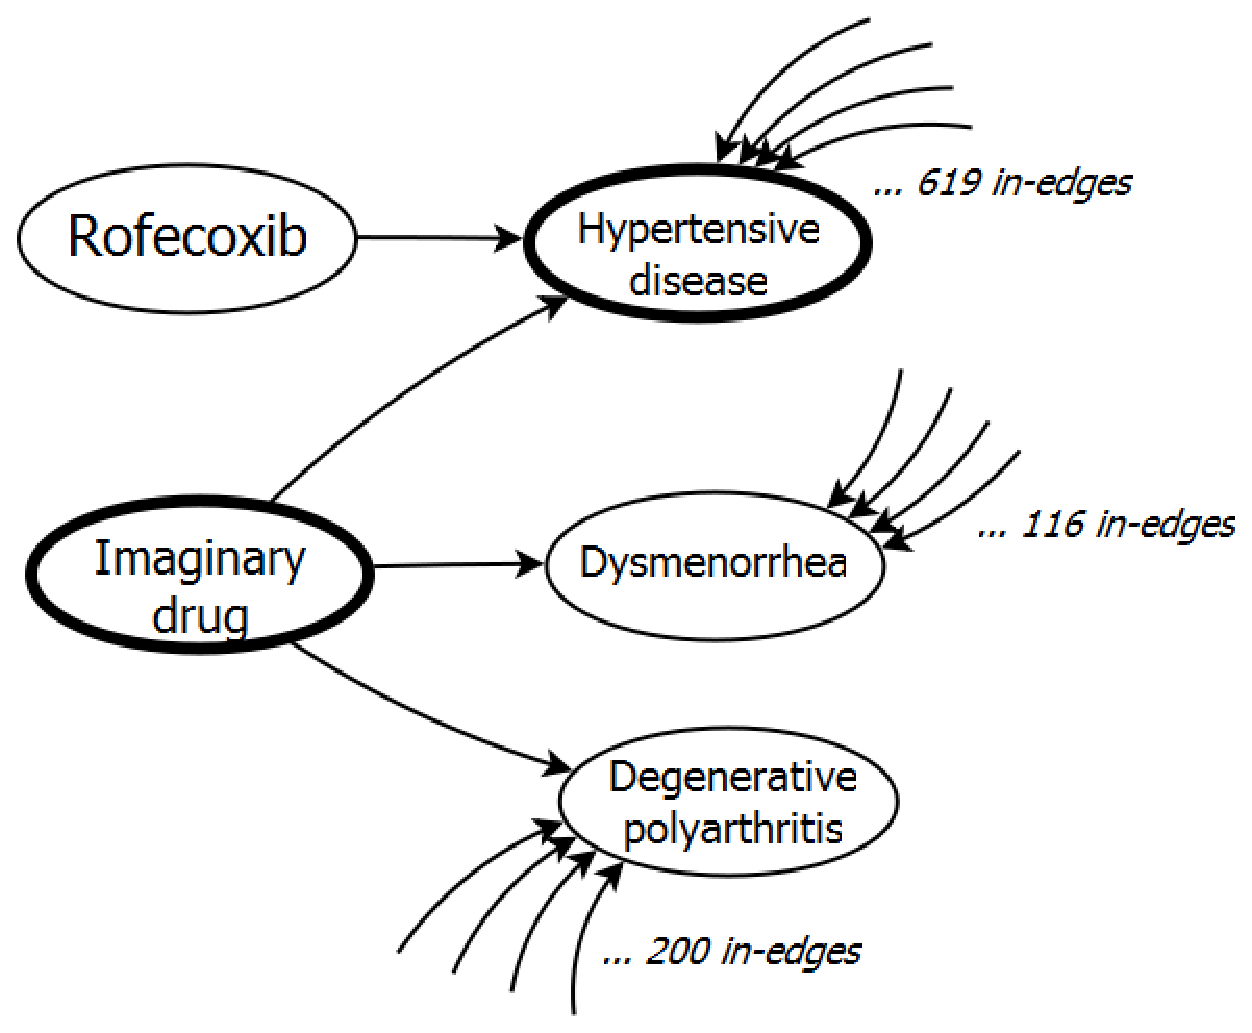
\includegraphics[width=.9\textwidth]{fig/may_treat_augmented.eps}
\end{minipage}
\caption[The may\_treat subgraph]{\label{fig:may_treat} The left-hand side of the figure shows the may\_treat subgraph of ground truth relationships between the drug Rofecoxib and two diseases. The right-hand side shows the may\_treat subgraph with some deliberately distorted information.}
\end{figure}

\begin{table*}[tbh]\scriptsize
\begin{center}
\begin{tabular}{ c || c  c || c  c }
\hline
        &   \multicolumn{2}{c||}{w/ noisy may\_treat only}    &   \multicolumn{2}{c}{w/ data and noisy may\_treat}\\
\hline
\hline
       	&   p(\%)   &   rank    &  p(\%)    &    rank    \\
\hline
$\langle Rofecoxib, degenerative~polyarthritis\rangle$       &   3.60e-3   &   555     &   8.14e-3    &   263    \\
$\langle Rofecoxib, dysmenorrhea\rangle$    &   1.54e-2   &   246     &   1.26e-3    &   1703   \\
\hline
\end{tabular}
\end{center}
\caption[Rankings of associations on the noisy may\_treat graph]{\label{tbl:salted_may_treat}Rankings of associations between Rofecoxib and two diseases on the noisy may\_treat graph (Figure~\ref{fig:may_treat} right) derived with and without data.}
\end{table*}

Conversely, we are also interested in learning whether the data graph can help discover patterns in the ontology graph. Figure~\ref{fig:may_treat} (left) shows a subgraph of the NDFRT ``may\_treat" relationship. Rofecoxib is asserted to treat two diseases, namely, dysmenorrhea and degenerative polyarthritis. And there are altogether 116 and 200 drugs that are known to treat dysmenorrhea and degenerative polyarthritis respectively (hence the in-degrees of the nodes). Applying our method on this graph with the query term ``Rofecoxib" yields a similarity-ranked list having degenerative polyarthritis and dysmenorrhea as the top two items. Since this result is the exact ground truth, there is no improvement to be made with the incorporation of the data graph. Therefore, we alter the ground truth graph with some deliberately distorted information, as is shown in Figure~\ref{fig:may_treat} (right), so that the may\_treat graph alone produces only inferior result. More specifically, we specify that Rofecoxib should treat hypertensive disease, the very diseases that is asserted to be treated by the most drugs (a total of 619). Then we add an imaginary drug to treat degenerative polyarthritis, dysmenorrhea, and hypertensive disease. In this way, the original direct connections between Rofecoxb and degenerative polyarthritis and dysmenorrhea become erroneously indirect and are obfuscated by some the noise of high degree nodes along the path. With this scenario, we hope to learn if the incorporation of data graph can correct the misinformation in ontologies.

Table~\ref{tbl:salted_may_treat} shows the result of ranks of the associations between Rofecoxib and degenerative polyarthritis and dysmenorrhea. The ranks of the associations drastically drop to the 555th and 246th respectively on the noisy graph from the top two on the original ground truth graph. This is mainly due to the large node, hypertensive disease, in the middle of the connections. However, with the combined data and may\_treat graph, we notice that the rank of Rofecoxib and degenerative polyarthritis increases to 263rd, while the rank of Rofecoxib and  dysmenorrhea decreases to 1703rd. This shows that the data graph endorses more strongly the association between Rofecoxib and degenerative polyarthritis. Indeed, although Rofecoxib are known to treat both degenerative polyarthritis and dysmenorrhea, the former is a much more popular usage. A search on the National Library of Medicine's PubMed database\footnotemark[1] for ``Rofecoxib and polyarthritis" returns 518 results, while ``Rofecoxib and dysmenorrhea" only returns 29. This result shows that the data graph can help correct misinformation in ontologies to some extent, and in a sense, it also gives a clue of how prior beliefs fit with reality.

\footnotetext[1]{\url{http://www.ncbi.nlm.nih.gov/}}

%We believe our results have demonstrated the utility of mining combined RDF bipartite graph of data and ontologies. Using the RDF bipartite graph as a unified representation, the incorporation of domain knowledge can be achieved by encoding the knowledge in the ontology or finding appropriate existing domain ontologies, then choose appropriately the relevant relationships that best suit the mining task.

\begin{comment}
\section{Discussion}
\label{sec:discussion}
We have demonstrated that using the proposed combined RDF bipartite graph incorporates both ontologies and data based on the user's desired weights for each component for finding semantically associated itemsets.

Developing scalable algorithms for semantic data mining is critically important. In our work, the healthcare dataset has grown beyond 100 billion triples and the size of the ontologies used are also large (SNOMED-CT has nearly 400,000 classes). The RWR method we describe works well for query-based node similarity, but it will not scale to generate full pair-wise node similarities at this tremendous scale.% because a calculation of eigenvectors of the Laplacian is required to derive the similarity measures, which is very expensive on large graphs.

While non-trivial practical problems associated with very large graphs cannot be completely avoided, our work makes it possible to leverage decades of work on graph-based methods in this effort to mine semantically associated data. The general strategy going forward is to employ approximation and develop parallelizable algorithms. Lin and Cohen~\cite{LinEtal2010ICML} proposed an approximation to a eigenvalue-weighted linear combination of all the eigenvectors, which can be achieved by performing a small number of matrix-vector multiplications.  The procedure results in a more scalable method called \emph{power iteration clustering} that finds a very low-dimensional data embedding using truncated power iteration on a normalized pair-wise similarity matrix of the data points. Zhao et al.~\cite{ZhaoEtal2011Eff} described the idea of \emph{graph coordinate systems}, which provides a fast embedding of large graphs into a hyperbolic space. The method parallelizes easily and efficiently locate shortest paths between node pairs, which relates well to the notion of commute time distance, which our RWR method seeks to elicit. Savas and Dhillon~\cite{SavasEtal2011Clu} introduced a novel framework called \emph{clustered low rank matrix approximation for massive graphs}. After a few intermediate steps, they are able to finally project an optimal, low rank approximation of the entire graph, thus including connections or edges between vertices from different clusters. We intend to extend these ideas to ontology-annotated hypergraphs.

The weighted hyperedges provide a great deal of flexibility to users who may prefer domain knowledge over data (or vice versa) and opens up new research questions on how to optimally learn the weights. In reality, the appropriate ratio for the edge weights is not only dependent on the size of graphs but also the graph configuration (depth, average degree, etc). Moreover, allowing users to specify the ratio of prior knowledge in ontologies versus inductive evidence from data enables us to discover empirically optimal configurations. We have performed exhaustive feature selection on classification algorithms for our healthcare dataset in the past, and we would also explore a few permutations on these hyperedge weights going forward. We can draw upon other works, such as, Tian et al.~\cite{Tian09}, who proposed an semi-supervised approach for classifying nodes in a graph based on a relatively small labeled set.

The RDF bipartite graph representation has limited expressivity compared to OWL itself. For example, domain, range and cardinality constraints are not straightforward to model.  One possible approach is to model domain constraints by explicitly describing the desired or acceptable walk (traversal sequence) in the RDF hypergraph. In this case, the recently proposed \emph{regular traversal expression} ~\cite{Marko10} technique may apply. However, their fast power-iteration approach for computing the stationary probability may not be applicable any more due to the label sequence constraint, but the Monte-Carlo simulation of the random walk may help to approximate the similarity measure.

We have showcased the utility of the RDF bipartite graph in mining \emph{semantically associated itemsets} and will explore other data mining tasks as well. For example, the classification task can be formulated as discovering the correct labels for unlabeled vertices in the weighted bipartite graph. Conceptually, the pair of nodes being ``close to'' one another shall share the same labels, which are consistent to one basic principle of semi-supervised learning, so the challenge is to define the closeness between two nodes. The clustering task can be viewed as a neighborhood formation for vertices on the data partition. Basically, for any closely related nodes, we group them together. Again, with an explicit similarity measure, possibly even the classical k-means in this case, could be directly applied to cluster the vertices.
\end{comment} 